\documentclass[tikz,border=2pt]{standalone}
\usepackage{amsmath,amssymb}
\usepackage{tikz}
\usetikzlibrary{arrows.meta}

\begin{document}
% A linear map sends the square grid to a grid of parallelograms: lines stay lines, the origin
% stays put, and sums and multiples are preserved.
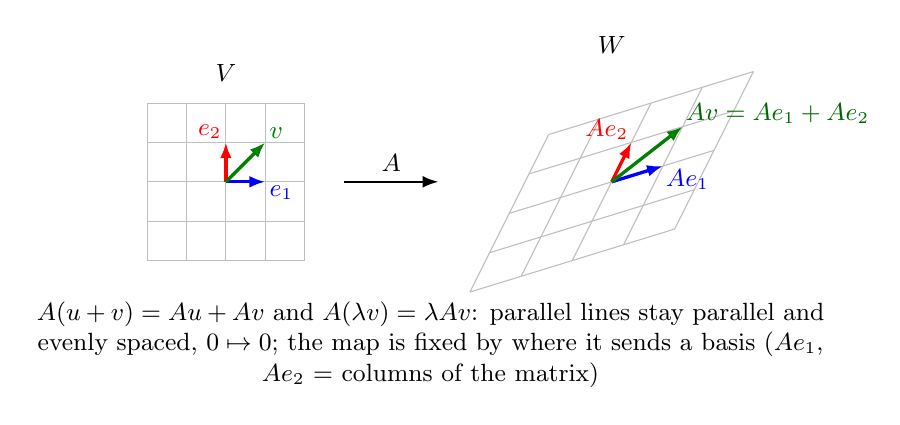
\begin{tikzpicture}[every node/.style={font=\small}, >={Latex[length=2mm]}]
	\foreach \i in {-2,...,2} {
		\draw[gray!50] (\i*0.5,-1) -- (\i*0.5,1);
		\draw[gray!50] (-1,\i*0.5) -- (1,\i*0.5);
	}
	\draw[->, blue, very thick] (0,0) -- (0.5,0) node[below right, inner sep=1pt] {$e_1$};
	\draw[->, red, very thick] (0,0) -- (0,0.5) node[above left, inner sep=1pt] {$e_2$};
	\draw[->, green!50!black, very thick] (0,0) -- (0.5,0.5) node[above right, inner sep=1pt] {$v$};
	\node[anchor=south] at (0,1.15) {$V$};
	\draw[->, thick] (1.5,0) -- (2.7,0) node[midway, above] {$A$};
	\begin{scope}[xshift=4.9cm, cm={1.3,0.4,0.5,1.0,(0,0)}]
		\foreach \i in {-2,...,2} {
			\draw[gray!50] (\i*0.5,-1) -- (\i*0.5,1);
			\draw[gray!50] (-1,\i*0.5) -- (1,\i*0.5);
		}
		\draw[->, blue, very thick] (0,0) -- (0.5,0);
		\draw[->, red, very thick] (0,0) -- (0,0.5);
		\draw[->, green!50!black, very thick] (0,0) -- (0.5,0.5);
	\end{scope}
	\node[blue, below right, inner sep=1pt] at (5.55,0.2) {$Ae_1$};
	\node[red, above left, inner sep=1pt] at (5.15,0.5) {$Ae_2$};
	\node[green!40!black, above right, inner sep=1pt] at (5.8,0.7) {$Av=Ae_1+Ae_2$};
	\node[anchor=south] at (4.9,1.5) {$W$};
	\node[anchor=north, align=flush center, text width=10cm] at (2.6,-1.4) {$A(u+v)=Au+Av$ and $A(\lambda v)=\lambda Av$: parallel lines stay parallel and evenly spaced, $0\mapsto0$; the map is fixed by where it sends a basis ($Ae_1$, $Ae_2$ = columns of the matrix)};
\end{tikzpicture}
\end{document}
